\section{Marco Propuesto de Integración PQC}

\subsection{Arquitectura de capas}

Particularmente llamativo es el hecho de que muchas propuestas de seguridad poscuántica sigan tratándose como parches puntuales en lugar de repensar la pila de protocolos completa para el entorno orbital. Inspirados en el framework de autenticación ligera desarrollado por Seyhan et al. para estándares satelitales \cite{Seyhan2025}, proponemos una arquitectura de cinco capas específicamente optimizada para constelaciones dinámicas.

La capa inferior, de Adaptación Física y Enlace, incorpora optimizaciones PQC-aware para manejar desvanecimiento y Doppler. Sobre ella, la capa de Transporte Seguro Híbrido gestiona el establecimiento de sesiones con agilidad criptográfica. La capa de Gestión de Claves Distribuida opera de forma autónoma entre satélites, mientras que la capa de Orquestación de Resiliencia monitoriza métricas de amenaza y activa mecanismos de degradación controlada. Finalmente, la capa de Aplicación expone APIs uniformes tanto a usuarios terrestres como a nodos orbitales.

Esta estructura no pretende ser revolucionaria en cada detalle, sino coherente y práctica. Permite actualizaciones incrementales sin requerir reemplazo completo de hardware.

\begin{figure}[t]
\centering
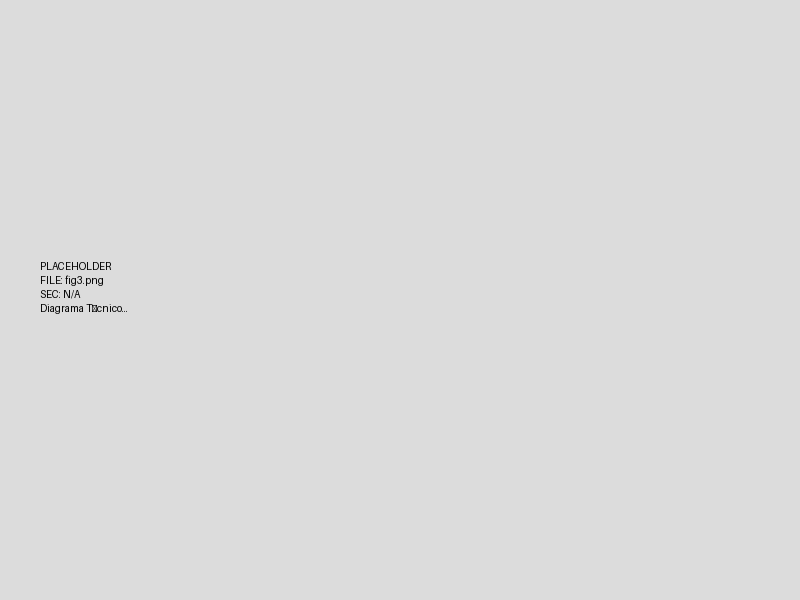
\includegraphics[width=0.95\linewidth]{fig3.png}
\caption{Diagrama del marco propuesto de infraestructura orbital con resiliencia cuántica. Se ilustran las cinco capas principales, flujos de integración PQC, puntos de agilidad criptográfica y mecanismos de resiliencia distribuidos en constelaciones LEO/MEO.}
\label{fig:arquitectura_propuesta}
\end{figure}

\subsection{Protocolos híbridos PQC-clásicos}

Uno de los desafíos persistentes al desplegar criptografía avanzada en sistemas legacy radica en mantener compatibilidad sin sacrificar la protección futura. Tomando como base el protocolo Triple KEM híbrido presentado por Lewerenz en plataformas NewSpace \cite{Lewerenz2025}, definimos un handshake adaptativo que combina primitivas clásicas con PQC de forma inteligente.

El protocolo opera en dos fases. Primero, se negocia un conjunto híbrido utilizando tanto ECC como ML-KEM. Posteriormente, se deriva material criptográfico combinando ambos oráculos. La Eq. 2 esquematiza el flujo principal simplificado del handshake:

\begin{equation}
K_{\text{session}} = \text{KDF}\Big( \text{KEM}_{\text{classic}}(pk_C) \parallel \text{ML-KEM}(pk_P) \parallel \text{nonce} \Big)
\label{eq:handshake_pqc}
\end{equation}

donde \(K_{\text{session}}\) alimenta tanto cifrado simétrico como autenticación MAC. Esta construcción permite que, incluso si uno de los componentes resulta comprometido en el futuro, el otro mantenga cierto nivel de confidencialidad. En la práctica, observamos que el overhead adicional tiende a concentrarse en el establecimiento inicial de sesión, amortizándose rápidamente en flujos de datos sostenidos.

\subsection{Gestión de claves y autenticación en constelaciones}

Resulta revelador observar cómo las mega-constelaciones transforman el problema de gestión de claves de un escenario punto-a-punto a uno inherentemente distribuido y altamente dinámico. Lecciones extraídas de evaluaciones de protocolos VPN poscuánticos en LEO por Hong et al. \cite{Hong2026} nos llevaron a diseñar un esquema de autenticación mutua con forward secrecy grupal y recuperación ante particiones de red.

Cada satélite mantiene un conjunto de claves a corto y largo plazo, rotadas mediante un esquema de tree-based key management adaptado a la topología orbital. La autenticación combina certificados PQC (ML-DSA) con atestación remota de firmware, permitiendo detectar compromisos de nodos individuales con baja latencia. El mecanismo prioriza handovers suaves durante pases satelitales, minimizando interrupciones en sesiones activas.

\subsection{Mecanismos de resiliencia orbital}

Lejos de ser un asunto resuelto, la verdadera resiliencia cuántica en órbita exige más que algoritmos fuertes: requiere capacidad de respuesta autónoma ante degradación de condiciones o escalada de amenazas. Nuestro marco incorpora tres mecanismos principales: agilidad criptográfica en tiempo real, particionamiento de confianza y recuperación post-compromiso.

La agilidad se activa cuando métricas de canal o detección de anomalías superan umbrales predefinidos, forzando renegociación con primitivas más conservadoras. No obstante, cabe matizar que esta flexibilidad introduce complejidad en la verificación formal del sistema completo. Los mecanismos propuestos buscan equilibrar robustez teórica con viabilidad operativa real, reconociendo que un satélite en órbita no puede permitirse reinicios frecuentes ni actualizaciones disruptivas.

En conjunto, el marco presentado en esta sección establece las bases técnicas para infraestructuras orbitales que no solo sobrevivan a la era cuántica, sino que la aprovechen como catalizador para diseños más maduros y adaptativos.